% !TEX program = xelatex
\DocumentMetadata{} % required for transparent package
\documentclass[11pt,aspectratio=169]{beamer}

% remove footcite numbers
\makeatletter
\def\@makefnmark{}
\makeatletter

\setbeamersize{text margin left=5mm,text margin right=5mm} 

\newcommand\focus[1]{%
	{\alert{\textbf{#1}}}
}

\usepackage{amsthm,amsmath,amssymb,braket,fontspec,unicode-math,fontenc,transparent}
\usepackage[absolute,overlay]{textpos}

\usetheme{moloch}
\setmainfont{SF Pro Display}
\setsansfont{SF Pro Display}
\setmathfont{Fira Math}
\setmathfont{latinmodern-math.otf}[range={frak,\bigcap,\bigcup}]

\usepackage[backend=bibtex,url=false,doi=false,style=authoryear]{biblatex}
\setbeamertemplate{bibliography item}{}
\bibliography{bib}
\AtBeginBibliography{\scriptsize}

\graphicspath{{./figures/}}

\setbeamerfont{title}{size=\LARGE\scshape}
\setbeamerfont{author}{size=\large}
\setbeamerfont{institute}{size=\large}
\setbeamerfont{date}{size=\large}
\setbeamerfont{frametitle}{size=\large\scshape}
\setbeamerfont{sectiontitle}{size=\small\scshape}

\title{Research Progress Report: 2023 - 2024}
\author{Abhirup Mukherjee}
\institute{
Department of Physical Sciences, IISER Kolkata, Mohanpur}

\begin{document}

\centering

\begin{frame}
\maketitle

\begin{textblock*}{0.3\textwidth}(0.5cm, 6.5cm)
	\includegraphics[width=0.4\textwidth]{epqm_logo_mod.jpeg}
	\hspace*{\fill}
	\includegraphics[width=0.4\textwidth]{dps_logo.jpeg}
\end{textblock*}
\hspace*{\fill}
\end{frame}

\begin{frame}{Acknowledgements}
	\flushleft
	\hspace*{20pt}
	\focus{Collaborators}: Debraj, Aashish, Arnabesh, Prof. N S Vidhyadhiraja, Prof. S Pujari\\
	\hspace*{20pt}
	\focus{Funding agencies}: IISER Kolkata, SERB
	\vspace*{\fill}

	\hspace*{\fill}
	\includegraphics[width=0.1\textwidth]{SERB.png}
	\hspace*{\fill}
	\includegraphics[width=0.1\textwidth]{dps_logo.jpeg}
	\hspace*{\fill}
	\includegraphics[width=0.1\textwidth]{epqm_logo_mod.jpeg}
	\hspace*{\fill}
\end{frame}

\begin{frame}{Publications and Ongoing Projects}
\focus{Published}\\[5pt]

\begin{minipage}{0.49\textwidth}
\begin{itemize}
	\item 2023 New J. Phys. 25 113011
	\item 2024 J. Phys. A: Math. Theor. 57 275401
\end{itemize}
\end{minipage}
\begin{minipage}{0.49\textwidth}
\begin{itemize}
	\item \transparent{0.4}{2022 Phys. Rev. B 105, 085119}
	\item \transparent{0.4}{2023 J. Phys.: Condens. Matter 35 315601}
\end{itemize}
\end{minipage}

\vspace*{\fill}

\focus{Currently in Progress}
\begin{itemize}
	\item Development of auxiliary model-based method for interacting electronics.
	\item Studies of the plateau-to-plateau transition in integer quantum hall systems.
\end{itemize}

\vspace*{\fill}

\focus{Ongoing Collaborations}

\begin{itemize}
	\item Breakdown of Kondo screening in presence of magnetic field [DD, AM, SL]
	\item Quantum critical Mott MIT in a three-orbital impurity model [AK, DD, AM, NSV, SL]
	\item Universal features of Kondo breakdown in quantum impurity models [DD, AM, SL]
	\item Search for non-Fermi liquid physics in mixed-valence regime of eSIAM [AS, AM, SL]
\end{itemize}
\end{frame}

\section{Ongoing Collaborations}

\begin{frame}{Breakdown of Kondo Screening in Presence of Magnetic Field}
\footcite{costi2000,Zhang2013}
\flushleft
Analysis of effect of impurity magnetic field on Kondo screening \\
(D Debata, A Mukherjee, S Lal) [{\it in preparation}]\\[10pt]

\begin{itemize}
	\item Models the effects of measurement on quantum system $+$ \focus{fermionic bath}
	\item Impurity undergoes localisation \focus{transition} at large \(B\)
	\item Critical point displays \focus{non-Fermi liquid} excitations.
\end{itemize}

\vspace*{\fill}
\centering
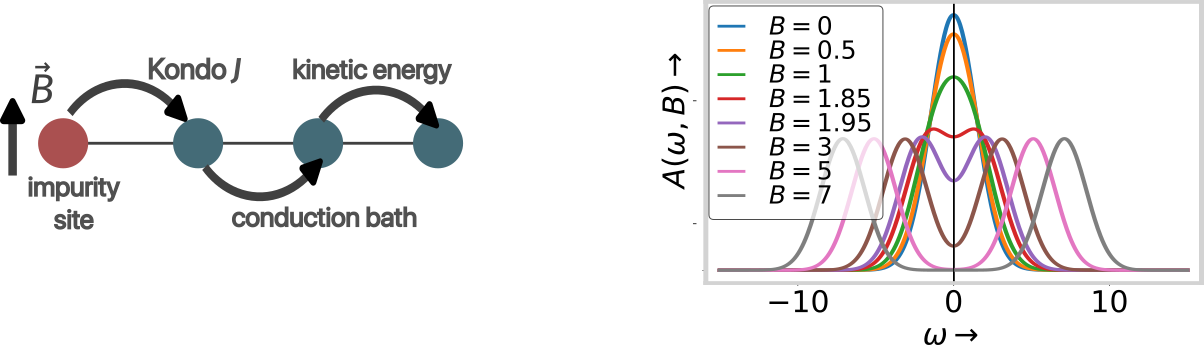
\includegraphics[width=0.8\textwidth]{kondoBFieldSpecFunc.pdf}

\end{frame}

\begin{frame}{Quantum critical Mott MIT in a Three-Orbital Impurity Model}
	\footcite{sujan2023,sudeshna2016}
\flushleft
Search for impurity model with a quantum critical phase intercepting a local MIT\\
(Aashish Kumar, D Debata, A Mukherjee, N. S. Vidhyadhiraja and S Lal) [{\it in preparation}]

\vspace*{\fill}
\begin{itemize}
	\item \focus{QC phase} obtained; gapless excitations involve composite paired objects
	\item Spectral function is pseudogapped at \(\omega \sim 0\).
	\item \focus{Self-energy} exponents characterise the non-Fermi liquid.
\end{itemize}

\vspace*{\fill}
\centering
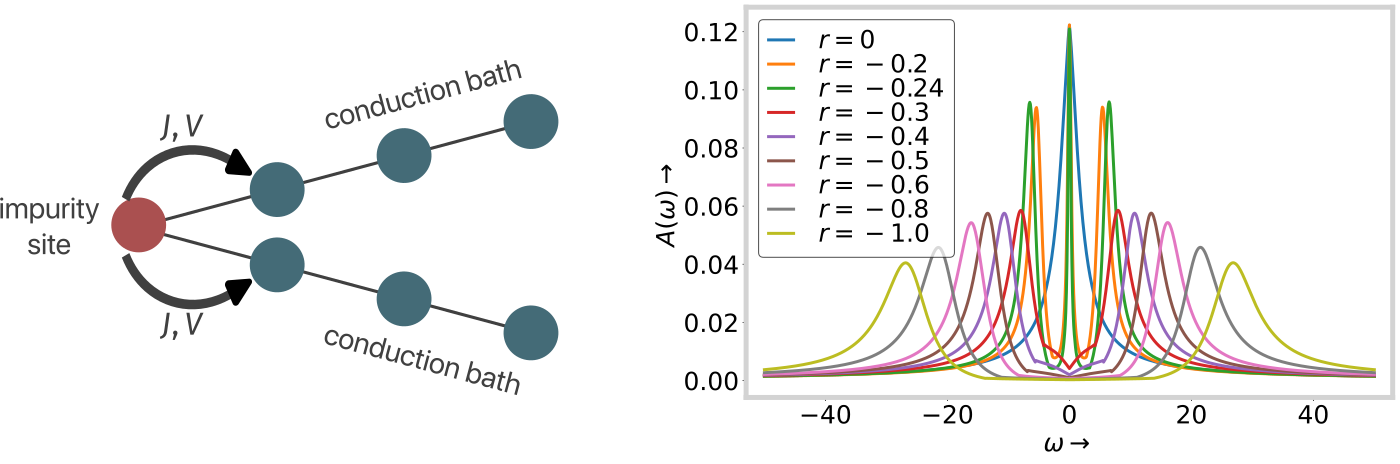
\includegraphics[width=0.8\textwidth]{threeOrbitalSpecFunc.pdf}
\end{frame}

\begin{frame}{Universal Features of Kondo Breakdown in Impurity Models}
\footcite{Mukherjee_2023,Patra_2023}
\flushleft
\vspace*{-20pt}
A unified framework for Kondo breakdown, in terms of entanglement measures\\
(D Debata, A Mukherjee, S Lal) [{\it in preparation}]\\[10pt]

\begin{itemize}
	\item Universal signatures of Kondo breakdown include \focus{partial magnetisation} and phase shift.
	\item Entanglement within the \focus{Kondo cloud} also suffers at Kondo breakdown.
\end{itemize}

\vspace*{\fill}
\centering
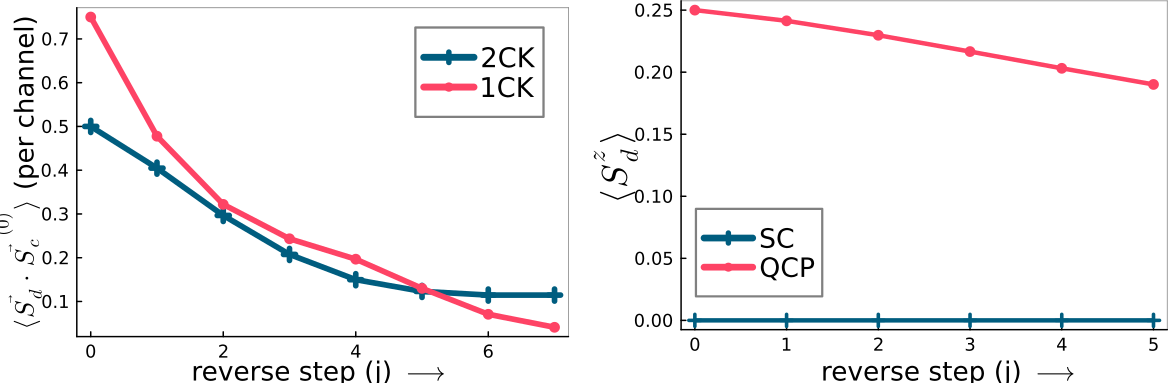
\includegraphics[width=0.7\textwidth]{compensation.pdf}
\end{frame}
	
\section{Project I: A New Auxiliary Model Approach to Systems of Interacting Electrons}

\begin{frame}{Broad Objectives}
	\footcite{keimer2015quantum,Sebastian2014,Norman1998}

	\vspace*{-20pt}
\begin{itemize}
	\item Designing a \focus{new method} by which to leverage quantum impurity models towards studying lattice models of interacting electrons\\[10pt]
	\item Using such a method to go after the \focus{Mott-Hubbard MIT} on the 2D square lattice\\[10pt]
	\item Capturing the effects of \focus{\(k-\)space anisotropy} on signatures near the transition\\[10pt]
	\item Studying the \focus{non-Fermi liquid behaviour} in the excitations near the transition
\end{itemize}

\hspace*{\fill}
\includegraphics[width=0.25\textwidth]{cupratesDiagram.png}
\hspace*{\fill}
\includegraphics[width=0.22\textwidth]{fermiArc.png}
\hspace*{\fill}
\end{frame}

\begin{frame}{Momentum-Resolved Renormalisation Group Flows}
\begin{minipage}{0.34\textwidth}
	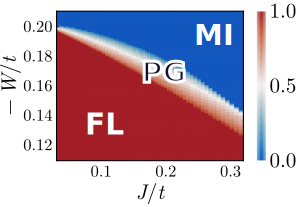
\includegraphics[width=\textwidth]{phaseDiagram.pdf}
\end{minipage}
\hspace*{\fill}
\begin{minipage}{0.45\textwidth}
	Hamiltonian RG equations of \\
	\focus{embedded e-SIAM}
	\[\Delta J^{(j)}_{{\bf k}_1, {\bf k}_2} = -\sum_{{\bf q} \in \text{PS}} \frac{J^{(j)}_{{\bf k}_2,{\bf q}} J^{(j)}_{{\bf q},{\bf k}_1} + 4J^{(j)}_{{\bf q}, {\bf \bar q}} W_{{\bf \bar q}, {\bf k}_2, {\bf k}_1, {\bf q}}}{\omega - \frac{1}{2}|\varepsilon_j| + J^{(j)}_{{\bf q}}/4 + W_{{\bf q}}/2}\]
\end{minipage}
\hspace*{\fill}
\begin{minipage}{0.19\textwidth}
	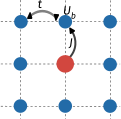
\includegraphics[width=\textwidth]{pWaveEsiam.pdf}
\end{minipage}

\vspace*{\fill}
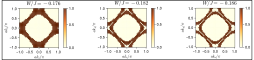
\includegraphics[width=0.9\textwidth]{scattProb.pdf}
	
\end{frame}

\begin{frame}{`Periodising' the Hamiltonian and Eigenstates}
	\footcite{stoyanova}
	\begin{minipage}{0.45\textwidth}
		Periodising the Hamiltonian creates a \focus{Hubbard-Heisenberg} model:
	\begin{equation*}\begin{aligned}
		\mathcal{H}_\text{tiled} =& \sum_{{\bf r}}T^\dagger({\bf r} - {\bf r}_d)\mathcal{H}_\text{aux}({\bf r}_d)T({\bf r} - {\bf r}_d)\\
	\end{aligned}\end{equation*}
	\end{minipage}
	\hspace{\fill}
	\begin{minipage}{0.45\textwidth}
		Wavefunctions can be related using a many-body \focus{Bloch's theorem}:
	\[\ket{\Psi_\text{gs}} = \frac{1}{\sqrt N}\sum_{{\bf r}_d} e^{i {\bf k}\cdot{\bf r}_d} \ket{\psi_\text{gs}\left({\bf r}_d\right)}\]

	\end{minipage}

	\vspace*{\fill}
	\(H_\text{tiled} = -\frac{\tilde t}{\sqrt{\mathcal{Z}}}\sum_{\left<{\bf r}_i, {\bf r}_j\right>;\sigma}\left(c^\dagger_{{\bf r}_i,\sigma}c_{{\bf r}_j,\sigma} + \text{h.c.}\right) + \frac{\tilde J}{\mathcal{Z}}\sum_{\left< {\bf r}_i, {\bf r}_j\right>}{\bf S}_{{\bf r}_i}\cdot{\bf S}_{{\bf r}_j} - \frac{\tilde U}{2}\sum_{\bf r}\left(\hat n_{{\bf r} , \uparrow} - \hat n_{{\bf r} , \downarrow}\right)^2\)

	\vspace*{15pt}
	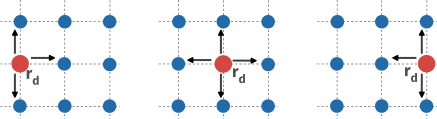
\includegraphics[width=0.8\textwidth]{periodisation.pdf}
	
\end{frame}

\begin{frame}{Periodising the Greens Functions}
	\footcite{kotliar2000,verret2022}
	\begin{minipage}{0.4\textwidth}
	Greens function = \\
	sum of 1-particle \focus{\(k-\)space} Greens functions starting from \focus{all sites} in impurity model.
	\end{minipage}
	\hspace{\fill}
	\begin{minipage}{0.54\textwidth}
	\begin{equation*}\begin{aligned}
		\tilde G({\bf r}; \tilde\omega) = \frac{1}{N}\sum_{{\bf k},{\bf r}_x} \left[e^{i \left({\bf k}- {\bf k}_0\right)\cdot\left({\bf r} - {\bf r}_x\right)}G_p\left({\bf r}_x;\omega + \varepsilon_{\bf k}\right) \right. \\
	\left. + e^{-i \left({\bf k}- {\bf k}_0\right)\cdot\left({\bf r} - {\bf r}_x\right)}G_h\left({\bf r}_x;\omega - \varepsilon_{\bf k}\right)\right]
	\end{aligned}\end{equation*}
	\end{minipage}

	\vspace*{\fill}
	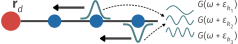
\includegraphics[width=0.8\textwidth]{greensFunc.pdf}

	\vspace*{\fill}
	\begin{minipage}{0.45\textwidth}
	Subsequently allows periodising spectral \\ 
	functions and self-energies
	\end{minipage}
	\hspace{\fill}
	\begin{minipage}{0.5\textwidth}
	\(\tilde A({\bf K}; \omega )= -\frac{1}{\pi}\text{Im}\left[\tilde G({\bf K}; \tilde\omega)\right]\)\\
	\(\tilde \Sigma({\bf K}; \omega) = \left(\tilde G^{(0)}({\bf K}; \tilde\omega)\right)^{-1} - \left(\tilde G({\bf K}; \tilde\omega)\right)^{-1}\)
	\end{minipage}
	
\end{frame}

\begin{frame}{Periodising Correlation Functions and Entanglement Measures}
	\footcite{Rozenberg2022,Meixner2024}
	\begin{minipage}{0.49\textwidth}
	\(k-\)space spin-spin correlation
	\begin{equation*}\begin{aligned}
	&\tilde{S}_\text{flip}({\bf K}_1, {\bf K}_2) = \\
	&\frac{1}{2}\left[\sqrt{\braket{S^+\left({\bf d}\right)S^-\left({\bf K}_2\right)}\braket{S^-\left({\bf d}\right)S^+\left({\bf K}_1\right)}} + \text{h.c.}\right]
	\end{aligned}\end{equation*}
	\end{minipage}
	\begin{minipage}{0.49\textwidth}
	\(k-\)space reduced density matrix
	\begin{equation*}\begin{aligned}
		&\overline\rho_{{\bf K},\sigma} = \frac{1}{2}\left[c^\dagger_{{\bf K},\sigma} \rho_\text{gs}({\bf r}_c) c_{{\bf r}_c,\sigma} + c^\dagger_{{\bf r}_c,\sigma} \rho_\text{gs}({\bf r}_c) c_{{\bf K},\sigma}\right] \\
		& + \text{h.c.}
	\end{aligned}\end{equation*}
	\end{minipage}
	
	\vspace{\fill}
	\centering
	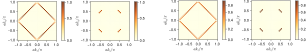
\includegraphics[width=\textwidth]{tilingEnt.pdf}
\end{frame}

\begin{frame}{Outstanding Questions}
	\begin{itemize}
		\item A better understanding of the mechanism of the pseudogap \focus{phase diagram}\\[10pt]
		\item Calculation of \focus{spectral functions} and self-energies\\[10pt]
		\item Characterisation of \focus{non-Fermi liquid} behaviour in the pseudogapped region
	\end{itemize}
\end{frame}

\section{Project II: Search for Punctured-Chern Topology at IQHE Transitions}

\begin{frame}{Broad Objectives}
\footcite{Khmelnitskii1983,Altland_Simons_2010,prangeGirvin1987}

\begin{itemize}
	\item Obtaining the \focus{IQHE phase diagram} from a model of 2D lattice electrons\\[10pt]
	\item Characterising the plateau-to-plateau transition \focus{critical point} through a topological invariant\\[10pt]
	\item Checking the robustness of our conclusions to the addition of \focus{disorder}
\end{itemize}
\vspace{\fill}

\hspace*{\fill}
\includegraphics[width=0.3\textwidth]{iqheRG.png}
\hspace*{\fill}
\includegraphics[width=0.33\textwidth]{iqheResis.png}
\hspace*{\fill}

\end{frame}

\begin{frame}{The Model}
	\begin{minipage}{0.45\textwidth}
	Non-interacting electrons, magnetic field, one-particle potential
	\[H = \frac{1}{2m}\left({\mathbf p} - e{\mathbf A({\mathbf r})}\right)^2 + V({\mathbf r})\]
	\end{minipage}
	\begin{minipage}{0.5\textwidth}
	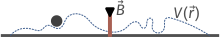
\includegraphics[width=\textwidth]{iqheModel.pdf}
	\end{minipage}

	\vspace{\fill}
	\begin{minipage}{0.45\textwidth}
		In the absence of \(V({\mathbf r})\), produces \\
		decoupled \focus{Landau levels} with\\
		large degeneracy.\\

		\(V({\mathbf r})\) leads to \focus{scattering} \\
		among these states.
	\end{minipage}
	\begin{minipage}{0.5\textwidth}
	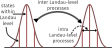
\includegraphics[width=\textwidth]{landauLevels.pdf}
	\end{minipage}
\end{frame}

\begin{frame}{URG Analysis of Intra Landau-level Processes}
\[
	H_n^* = \sum_{\varepsilon_{n,\alpha} \sim 0}\varepsilon_{n,\alpha} c^\dagger_{n, \alpha} c_{n,\alpha} + \sum_{|\varepsilon^*_{n,\alpha}| > \Delta^*}\varepsilon^*_{n,\alpha}c^\dagger_{n,\alpha} c_{n,\alpha} + \sum_{\varepsilon_{n,\alpha_1}, \varepsilon_{n,\alpha_2} \sim 0}L_{\alpha_1,\alpha_2}^*(n)\left(c^\dagger_{n, \alpha_1}c_{n,\alpha_2} + \text{h.c.}\right)
\]
States within a window are \focus{attracted} towards central state, with relevant forward scattering among them.

\begin{minipage}{0.4\textwidth}
	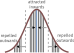
\includegraphics[width=\textwidth]{intraLL.pdf}
\end{minipage}
\hspace*{\fill}
\begin{minipage}{0.4\textwidth}
	\includegraphics[width=\textwidth]{intraLL_epsRG.pdf}
\end{minipage}
\end{frame}

\begin{frame}{URG Analysis of Inter Landau-level Processes}
	\footcite{cain2003,cain2005}
\begin{minipage}{0.45\textwidth}
Landau levels are repelled away from chemical potential (\focus{stability}).\\

LLs below chemical potential are decoupled and filled. 
\end{minipage}
\hspace*{\fill}
\begin{minipage}{0.4\textwidth}
	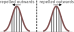
\includegraphics[width=\textwidth]{interLL.pdf}
\end{minipage}

\vspace{30pt}
\begin{minipage}{0.45\textwidth}
	\focus{Insulating phase}\\
	No longitudinal transport. \\
	Central state allows transverse transport.
\end{minipage}
\hspace*{\fill}
\begin{minipage}{0.45\textwidth}
	\focus{Critical point}\\
	Marginal scattering processes at Fermi level. Lead to longitudinal resistivity.
\end{minipage}
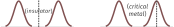
\includegraphics[width=0.8\textwidth]{effectiveTheoriesIQHE.pdf}
\end{frame}

\begin{frame}{Outstanding Questions}
	\begin{itemize}
		\item Description of the metal obtained at the \focus{critical point} (self-energy, etc.).\\[10pt]
		\item \focus{Topological invariant} to characterise the critical point (Chern number, etc.) \\[10pt]
	\end{itemize}
\end{frame}

\section{Future Plans}

\begin{frame}{Future Plans}
	\begin{itemize}
		\item Finish the embedded eSIAM project and the IQHE projects.
		\item Study heavy-fermion physics using auxiliary mode approach (simple extension of the embedded eSIAM project).
	\end{itemize}

	\vspace*{\fill}

	\hrule

	\vspace*{\fill}
	\Large{\bf Thank You!}
\end{frame}

\end{document}
